





\documentclass[12pt,letterpaper,notitlepage]{article}
\usepackage{graphicx}
\usepackage{epsfig,epsf}
\usepackage{epstopdf}
\usepackage{curves}
\usepackage{hyperref}
% The following packages are important as they allow to write certain mathematical expressions.
\usepackage{amsmath}
\usepackage{amssymb}
\usepackage{color}
% To write a code in a LaTeX document you need:
\usepackage{listings}
\definecolor{dkgreen}{rgb}{0,0.6,0}
\definecolor{dkblue}{rgb}{0,0.0,0.6}
\definecolor{dkred}{rgb}{0.9,0.0,0.1}
%% Own definitions:
\newcommand{\BEq}{\begin{eqnarray}}
\newcommand{\EEq}{\end{eqnarray}}
\newcommand{\BEqn}{\begin{eqnarray*}}
\newcommand{\EEqn}{\end{eqnarray*}}
\newcommand{\BM}{\begin{subequations}}
\newcommand{\EM}{\end{subequations}}
\newcommand{\BEqM}{\begin{subequations}\begin{eqnarray}}
\newcommand{\EEqM}{\end{eqnarray}\end{subequations}}
\newcommand{\Bitem}{\begin{itemize}}
\newcommand{\Eitem}{\end{itemize}}
\newcommand{\Ben}{\begin{enumerate}}
\newcommand{\Een}{\end{enumerate}}
%% Greek letters:
\renewcommand{\a}{\alpha}
\renewcommand{\b}{\beta}
\newcommand{\D}{\Delta}
%% Colors:
\newcommand{\TB}[1]{\textcolor{blue}{#1}}
\newcommand{\TR}[1]{\textcolor{red}{#1}}
\newcommand{\bm}[1]{\mbox{\boldmath $#1$}}
\newcommand{\non}{\nonumber\\}
%% Some simplified expressions:
\def\eps{\varepsilon}
\def\r{\right}
\def\l{\left}
\def\p{\partial}
\def\d{\delta}
\newcommand{\ta}{\mbox{$\theta$}}
\newcommand{\ve}{\mbox{${\cal E}$}}
\newcommand{\etab}{\bar{\eta}}
\newcommand{\sg}{\tilde{\sigma}}
\newcommand{\tap}{\mbox{$\theta'$}}
\newcommand{\tta}{\mbox{$\tilde{\theta}$}}
\newcommand{\ttap}{\mbox{$\tilde{\theta}'$}}
\newcommand{\taz}{\mbox{$\theta_0$}}
\newcommand{\phip}{\mbox{$\phi'$}}
\newcommand{\tphi}{\mbox{$\tilde{\phi}$}}
\newcommand{\tphip}{\mbox{$\tilde{\phi}'$}}
\newcommand{\ty}{\mbox{$\tilde{y}$}}
\newcommand{\gb}{\mbox{$\bar{\gamma}$}}
\newcommand{\gone}{\mbox{$\gamma_1$}}
\newcommand{\gtwo}{\mbox{$\gamma_2$}}
\newcommand{\phiz}{\mbox{$\phi_0$}}
\newcommand{\Nf}{\mbox{$N_f$}}
\newcommand{\Nv}{\mbox{$N_v$}}
\newcommand{\qt}{\mbox{$\tilde{q}$}}
\newcommand{\qa}{\mbox{$q_\alpha$}}
\newcommand{\tqa}{\mbox{$\tilde{q}_\alpha$}}
\newcommand{\dqa}{\mbox{$\delta q_\alpha$}}
\newcommand{\pqa}{\mbox{$\partial_{u} q_\alpha$}}
\newcommand{\pqta}{\mbox{$\partial_{u} \tilde{q}_\alpha$}}
\newcommand{\pdqa}{\mbox{$\partial_{u}\delta q_\alpha$}}
\newcommand{\sn}{\mbox{${\rm sn}$}}
\newcommand{\cn}{\mbox{${\rm cn}$}}
\newcommand{\dn}{\mbox{${\rm dn}$}}
\newcommand{\cd}{\mbox{${\rm cd}$}}
%%% Creation, destruction operators:
\newcommand{\cks}{\mbox{$c_{{\bf k},\sigma}$}}
\newcommand{\cksd}{\mbox{$c_{{\bf k},\sigma}^\dagger$}}
\newcommand{\cku}{\mbox{$c_{{\bf k},\uparrow}$}}
\newcommand{\ckd}{\mbox{$c_{-{\bf k},\downarrow}$}}
\newcommand{\ckud}{\mbox{$c_{{\bf k},\uparrow}^\dagger$}}
\newcommand{\ckdd}{\mbox{$c_{-{\bf k},\downarrow}^\dagger$}}

\begin{document}

\lstset{language=Fortran,tabsize=4,numbers=left,numberstyle=\tiny,basicstyle=\ttfamily\small\color{dkblue},stringstyle=\ttfamily\color{blue},keywordstyle=\rmfamily\color{dkred}\bfseries\emph,backgroundcolor=\color{white},commentstyle=\color{dkgreen}}




\title{%
	Energy States of 1D Harmonic Oscillator \\
\large Computional Physics - Phys 562}
\author{Benjamin Deutsch  \\
Department of Physics\\
California State University Long Beach}
\date{\today }

  
\maketitle



\begin{abstract}
Here we will utilize the Fortran 95 Programming environment to execute a recursive hermitian polynomial, on a 1 dimensional wave equation. From here we extract and plot function curves for the ground energy level, and sequential excited states, up to the tenth quantized regime.        
\end{abstract}

\section{Introduction}

A 1D harmonic oscillator can be visually represented a string of particles usually atoms, contained within and infinite square well. This allows particles to react to each other, but never escape their enclosure. The resulting motion is vibrating harmonically, or with a given energy. Each particles does not transfer energy along the string, as is the case in a standing wave, however the system maintains a quantized energy. This energy is even represented at A(0), giving meaning to the statement ground state energy, clearly not a zero value. Quantum mechanics guides understanding for the ladder operations, raising as well as lowering these vibrational states, but only by given discrete rungs. It is worth noting these levels, hold true physical meaning so lowering energy below the ground state is erroneous, and likewise negative values . These harmonic states exist in all physical material and are cornerstone to many fundamental theories. Exploration in to the mathematical properties of the wave equation of state is non-trivial for any physical science student, and the automation of a programming language, should reveal much about the recursive nature of the imperative equation. 



\section{The Math and Theory}

We will be looking at a 1D Harmonic oscillator for this assignment, which at present cannot be readily placed into the computer. 

	\begin{equation}
		\psi_n(x) = \frac{1}{\sqrt{2^n\,n!}} \cdot \left(\frac{m\omega}{\pi \hbar}\right)^{1/4}\cdot e^{
		- \frac{m\omega x^2}{2 \hbar}} \cdot H_n\left(\sqrt{\frac{m\omega}{\hbar}} x \right)
	\end{equation}
\\
Here, we can utilize the properties of the Hermite polynomials, 
\\
\begin{equation}
	H_{n+1}(x)=2xH_n(x)-2nH_{n-1}(x)
\end{equation}	
\\
Here we can collect dependents of $H_n$ 
\\
	\begin{equation}
		r = \sqrt{\frac{m\omega}{\hbar}} x
	\end{equation}
\\
	\begin{equation}
		\psi_n(x) = \frac{1}{\sqrt{2^n\,n!}} \cdot \left(\frac{m\omega}{\pi \hbar}\right)^{1/4}\cdot e^{
	-	 \frac{m\omega x^2}{2 \hbar}} \cdot H_n(r)
	\end{equation}
\\
Through some substitution;
\\
\BM
	\begin{align}
		H_n(r)={\sqrt{2^n\,n!}} \cdot \left(\frac{\pi \hbar}{m\omega}\right)^{1/4}\cdot e^{ \frac{m\omega x^2}{2 \hbar}} \cdot \psi_n(x)\\
		H_n(r)={\sqrt{2^n\,n!}} \cdot \left(\frac{\pi \hbar}{m\omega}\right)^{1/4}\cdot e^{ \frac{m\omega x^2}{2 \hbar}} \cdot \psi_n(x)\\
		H_n(r)={\sqrt{2^n\,n!}} \cdot \left(\frac{\pi \hbar}{m\omega}\right)^{1/4}\cdot e^{ \frac{m\omega x^2}{2 \hbar}} \cdot \psi_n(x)
	\end{align}
\EM 
\\
	\begin{equation}
		\psi_{n+1}(x)=2r\frac{\sqrt{2^{n} n!}}{\sqrt{2^{n+1}(n+1)!}}\psi_n (x) - 2n\frac{\sqrt{2^{n-1} (n-1)!}}{\sqrt{2^{n+1}(n+1)!}}\psi_{n-1}(x) 
	\end{equation}
\\
	\begin{equation}
		\psi_{n+1}(x)=2r{\sqrt{\frac{1}{2(n+1)}}}\psi_n (x) - {\sqrt{\frac{n}{(n+1)}}}\psi_{n-1} (x) 
	\end{equation}
\\
\\

At the end we have derive a recursive function which solely depends on the psi component, which at the same time has completely absorb the hermitian terms. 

From this point we can instruct the computer straightforwardly to attempt the recursion. 

\section{The code}

For all Fortran code we must begin with the variables, all terms used here in this program are define in the heading, as real, or integer. The only exception being the real dimensional term, which creates an array of entries of psi to be placed. 

In retrospect we can compile the code in a few different ways, my attempt with rudimental knowledge assembled a series of do loops nest within each other, more about this will be examined below. A slightly more advance code would use a subroutine function, meaning in which the wave equations would be expressed solely in terms of the hermitian polynomial subroutine and only then called into a do loop for discrete energy evaluations. The benefit for this method is the the operations needed can be called up for any selected energies or problem at the time, without affecting the entire code. 

For the nested do loops it is far simpler to explain from the inside outside. The recursive nature of the equations leaves only two necessary conditions to be fulfilled, one the function must initialized at zero and secondly, the recursive formulate must itinerate with steps following the pervious entries,  e.i. (n-1).
The second loop then takes these Psi entries and contrast them against number line spanning -500 to 500 on the x axis. The resulting wave is then subjected to the third and outermost loop where each new energy is raised giving an ascending scale of wave-energy plots for the 10 states called for. 

Each of the functions are then written to a separate file, where post run they can then be compiled.

\section{Results and Conculsion}

	\begin{figure}[htb]
		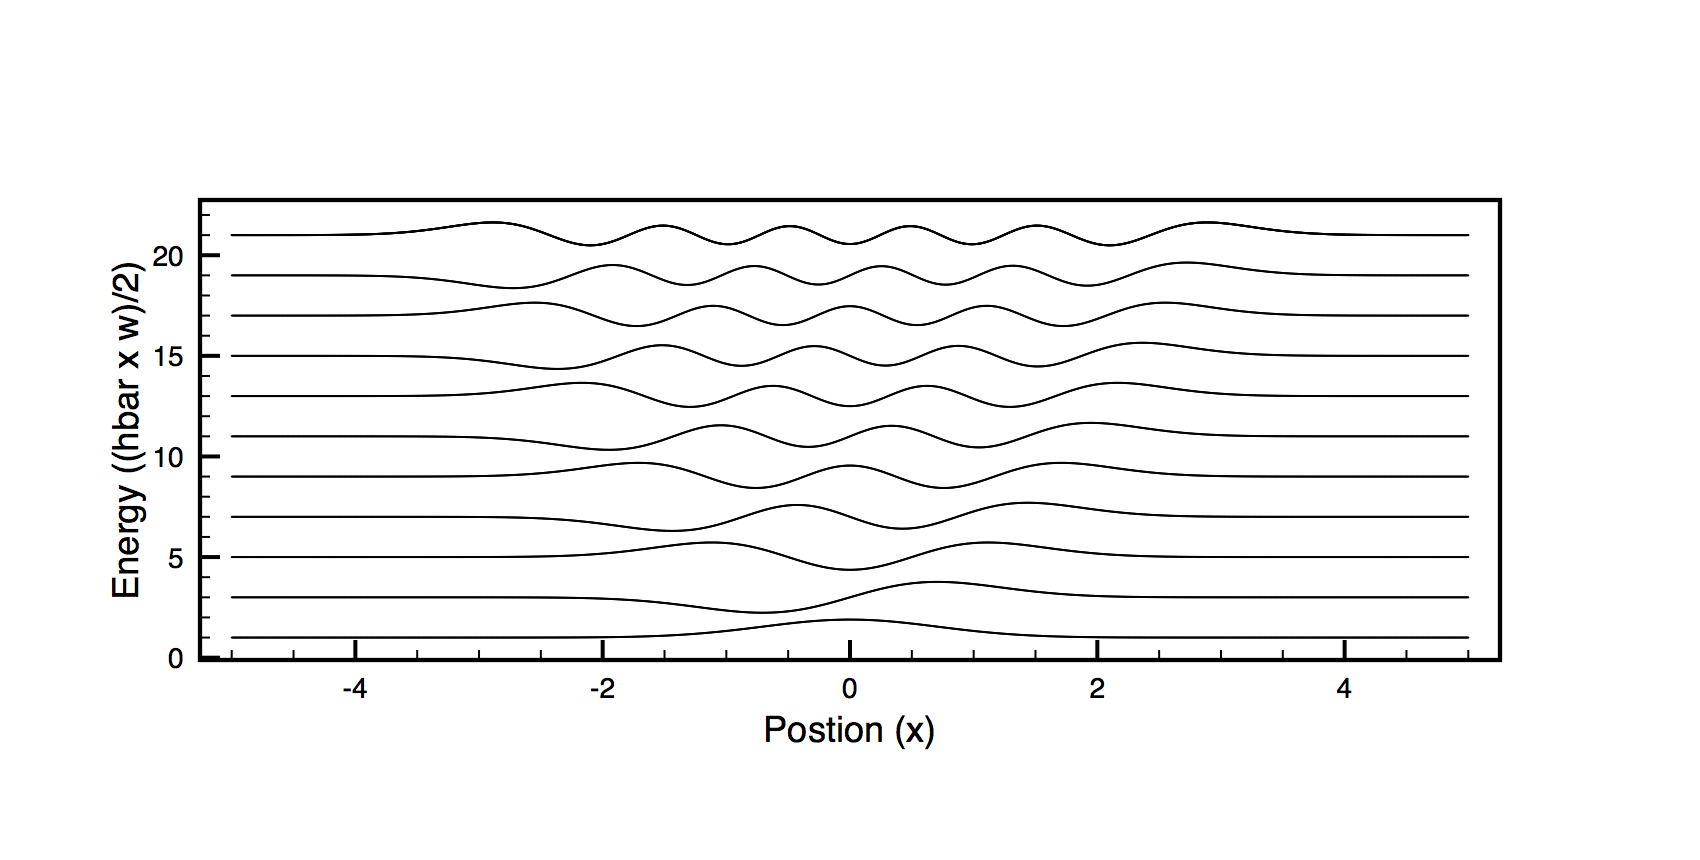
\includegraphics[width=1.\textwidth]{energies.png}
	\end{figure}

As the graph above indicates we can see a clearly quantized system of energies. Another item of consistency is the nearly flat measurements at the boundaries of the plot we can assume this is because of the parabolic nature of the harmonic energies growing with function of one half the pervious wavelength.

The results found here, agree strongly with exterior findings ei eigenstates of a quantum harmonic oscillator.  


\begin{thebibliography}{}


 \bibitem{1}
	Z.~Papp and A.~Bill, {\it Computational Physics Lecture Notes}, California State University Long Beach.

\end{thebibliography}




\end{document}








